\subsection{Number of Hops per Route}

We want to look at traceroute measurements. The first thing we analyze is the
average number of hops per traceroute measurement. For that, we use the RIPE
Atlas built-in traceroute measurements. Figure~\ref{fig:hops-per-measument}
shows the histogram of hops for Canada, the United~Kingdom, France, and
Germany. The countries were chosen due to the completeness of the data. Similar
results were found when looking at other countries.

\begin{figure}
	\centering
	\begin{subfigure}[b]{0.48\linewidth}
		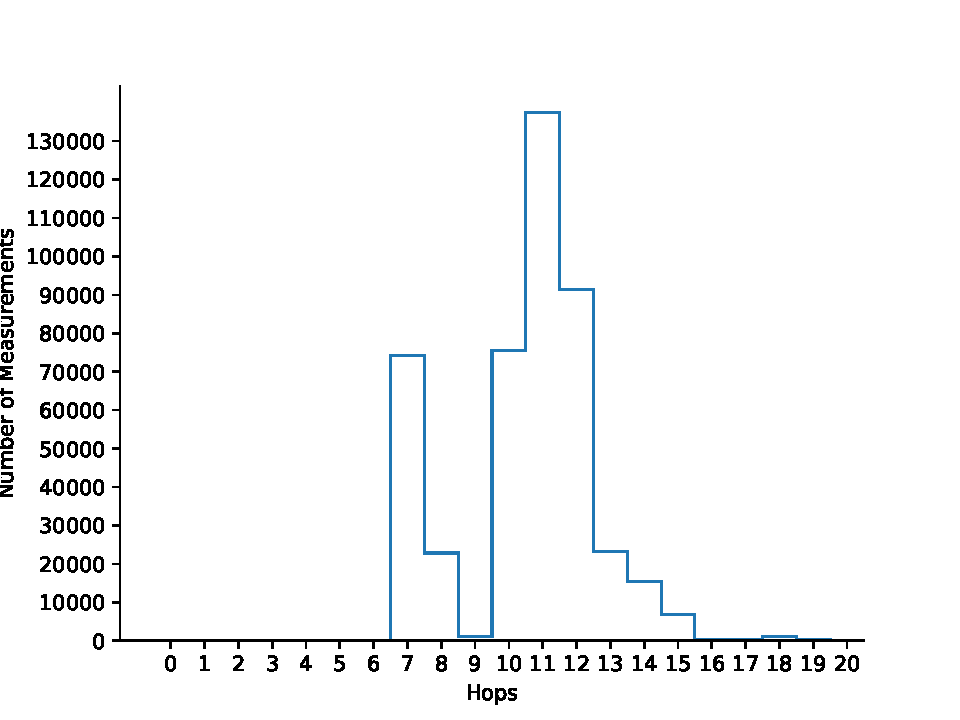
\includegraphics[width=\linewidth]{chapters/4-results/traceroute/img/hops_CA.pdf}
		\caption{Canada}
	\end{subfigure}
	\begin{subfigure}[b]{0.48\linewidth}
		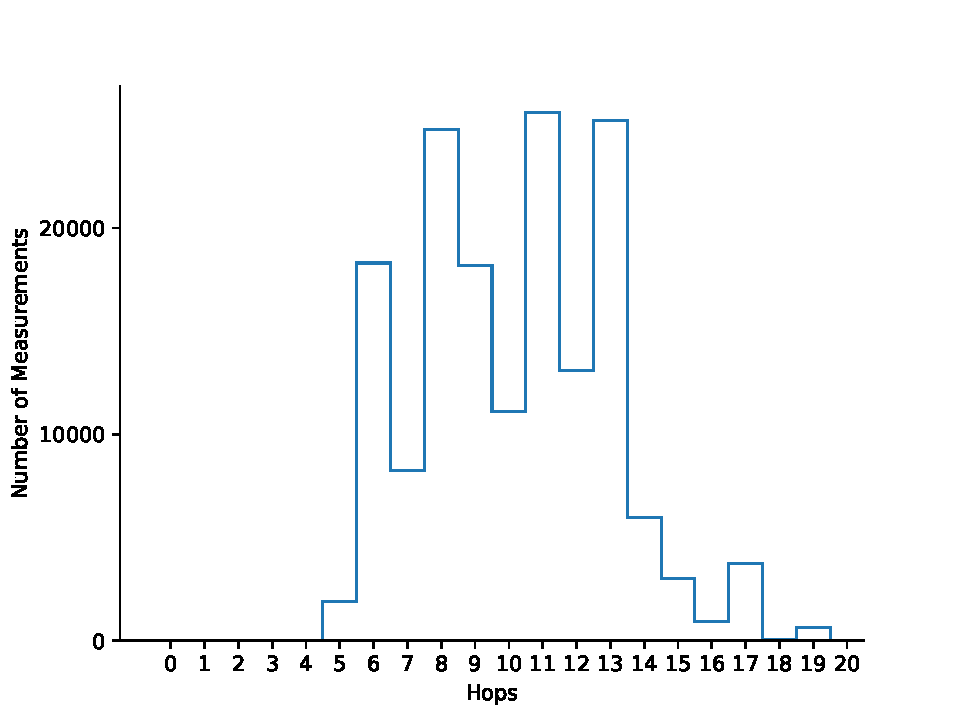
\includegraphics[width=\linewidth]{chapters/4-results/traceroute/img/hops_PH.pdf}
		\caption{Philippines}
	\end{subfigure}
	\begin{subfigure}[b]{0.48\linewidth}
		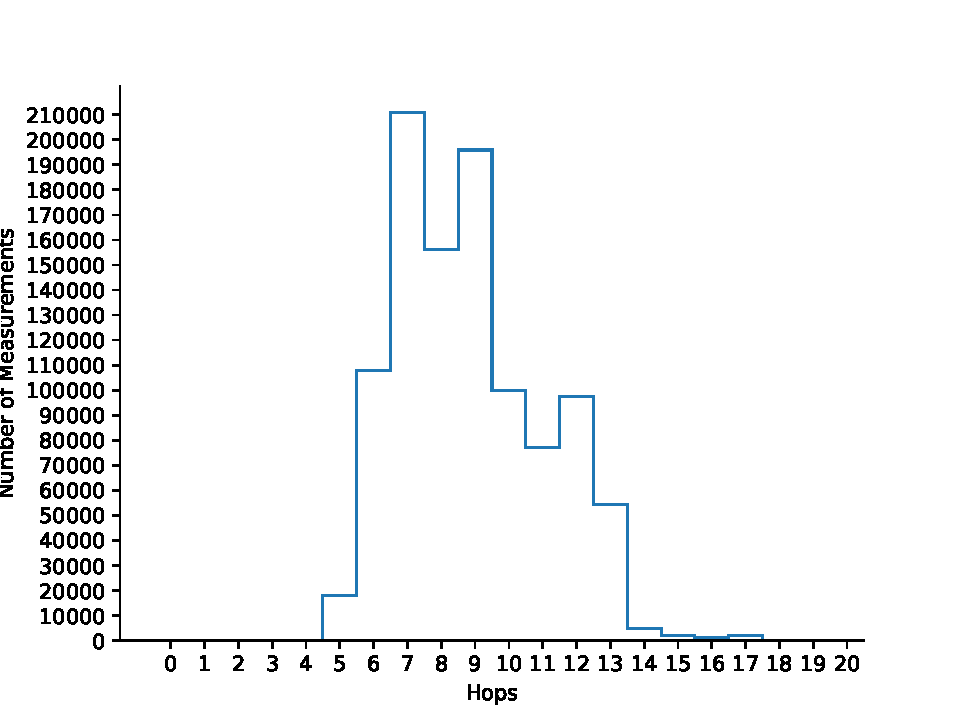
\includegraphics[width=\linewidth]{chapters/4-results/traceroute/img/hops_FR.pdf}
		\caption{France}
	\end{subfigure}
	\begin{subfigure}[b]{0.48\linewidth}
		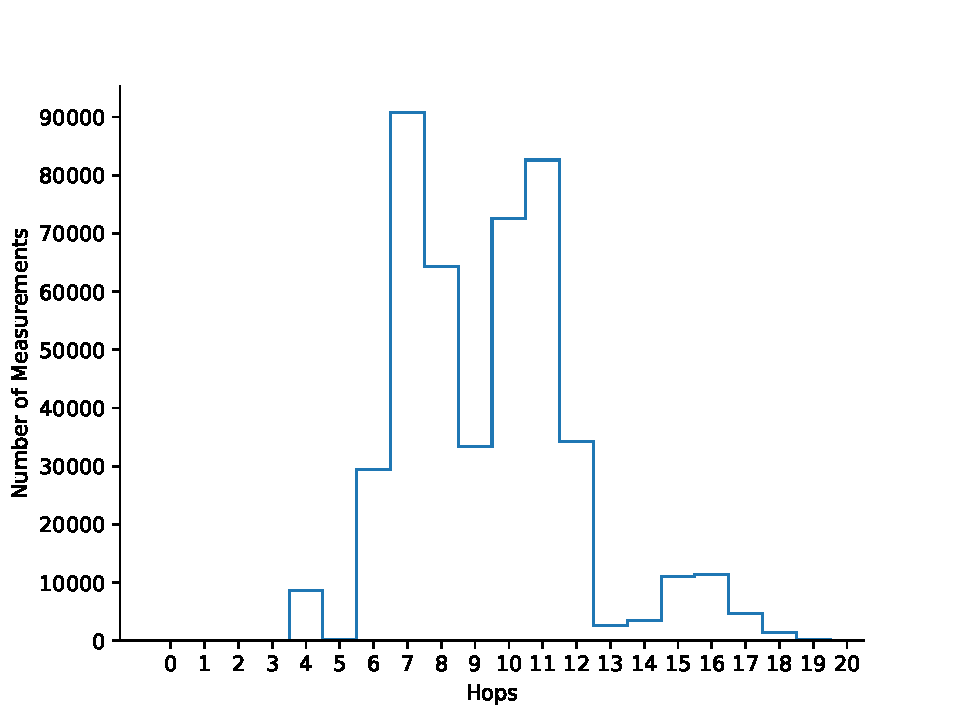
\includegraphics[width=\linewidth]{chapters/4-results/traceroute/img/hops_DE.pdf}
		\caption{Germany}
	\end{subfigure}
	\caption{Histogram of Hops the Traceroute Measurement took.}
	\label{fig:hops-per-measument}
\end{figure}

The histograms show that most routes take between seven and fourteen hops.
It is interesting to note that the histograms show a similar pattern compared
to the histogram for TLS handshake latencies that are shown in
Chapter~\ref{sec:latency-wholerange}. Both histograms have a pattern that
spikes at two points. We assume that there a specific reason for this
correlation that is part of the Starlink network.

\subsection{Latency per Hop}

We want to a closer look on how Starlink latency behaves in each hop. To do so,
we looked at each hop of the built-in measurements of RIPE~Atlas and the change
in round trip time from hop to hop. Figure~\ref{fig:latency-change-per-hop-1}
and \ref{fig:latency-change-per-hop-2} show how the round trip time measured in
the traceroute measurement behaves in consecutive hops. It is important to note
that in rare cases the RTT does not increase with more hops, as traceroute
measurements work with repetitive measurements that might yield inconsistent
results in consecutive runs. Also, we noticed a severe difference among the
target root servers. Therefore, we additionally differentiated by target. The
target is defined by RIPE Atlas in their documentation by measurement
ID\footnote{See
	\href{https://atlas.ripe.net/docs/built-in-measurements/\#traceroute-5-000-6-999}{RIPE Atlas Built-In Traceroute Measurements}}.
For this chapter, we focused on the measurement 5001 (traceroutes to
k.root-servers.net). Further figures are listed in the appendix (Figures
\ref{fig:latency-change-per-hop-appendix-1} --
\ref{fig:latency-change-per-hop-appendix-16}).

\begin{figure}
	\centering
	\begin{subfigure}[b]{\linewidth}
		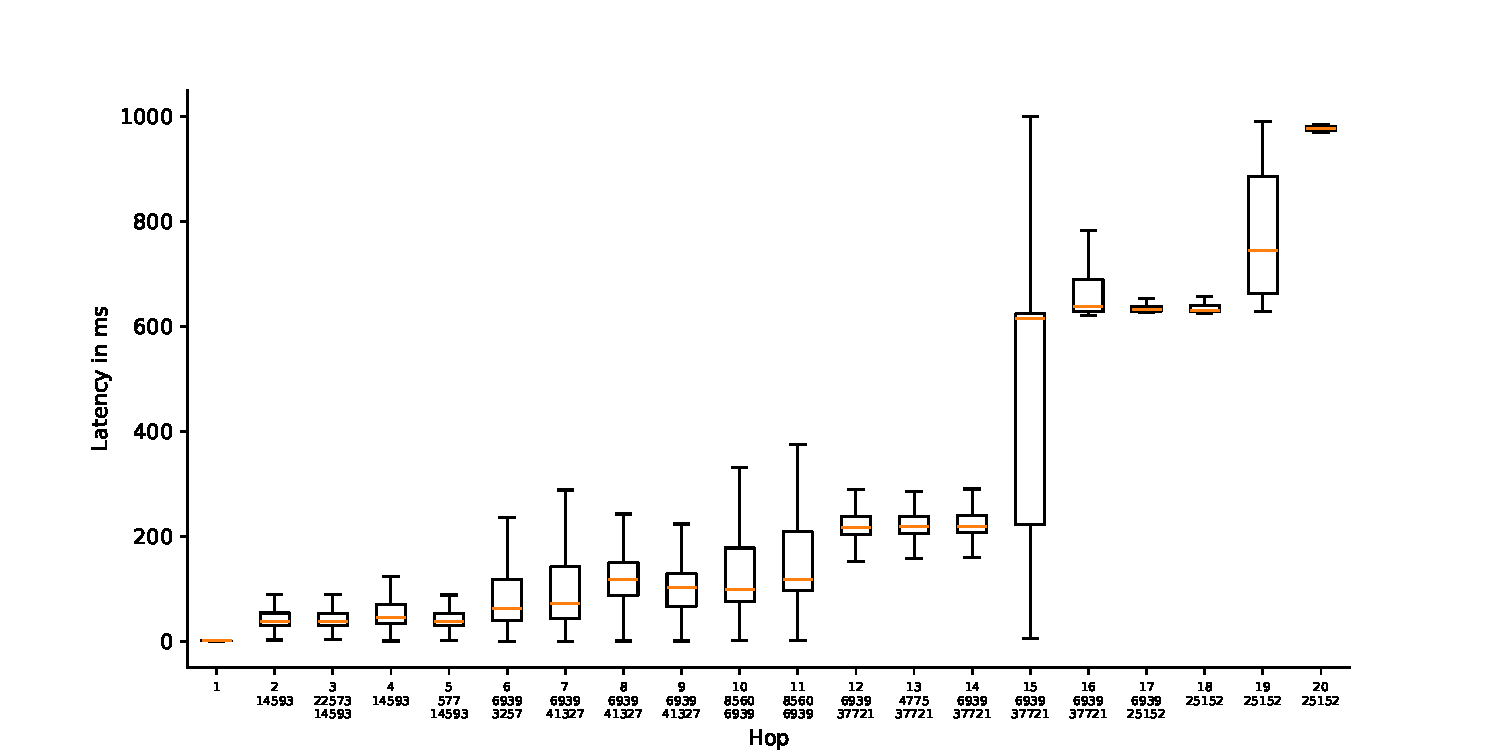
\includegraphics[width=\linewidth]{chapters/4-results/traceroute/img/latency-per-hop-CA-5001.pdf}
		\caption{Canada}
		\label{fig:latency-change-per-hop-1-ca}
	\end{subfigure}
	\begin{subfigure}[b]{\linewidth}
		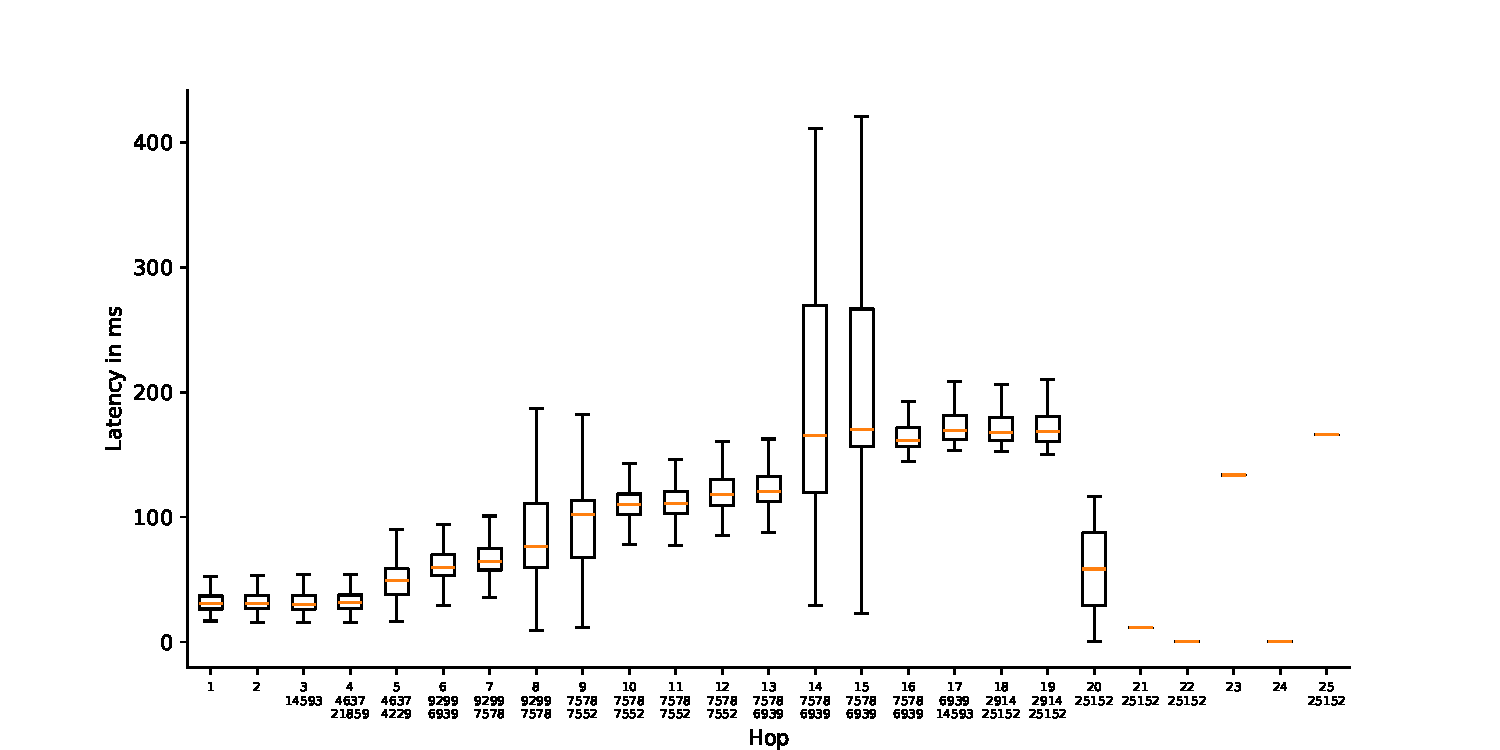
\includegraphics[width=\linewidth]{chapters/4-results/traceroute/img/latency-per-hop-PH-5001.pdf}
		\caption{Philippines}
	\end{subfigure}
	\caption{Latencies per Hop in Canada and Philippines}
	\label{fig:latency-change-per-hop-1}
\end{figure}

\begin{figure}
	\centering
	\begin{subfigure}[b]{\linewidth}
		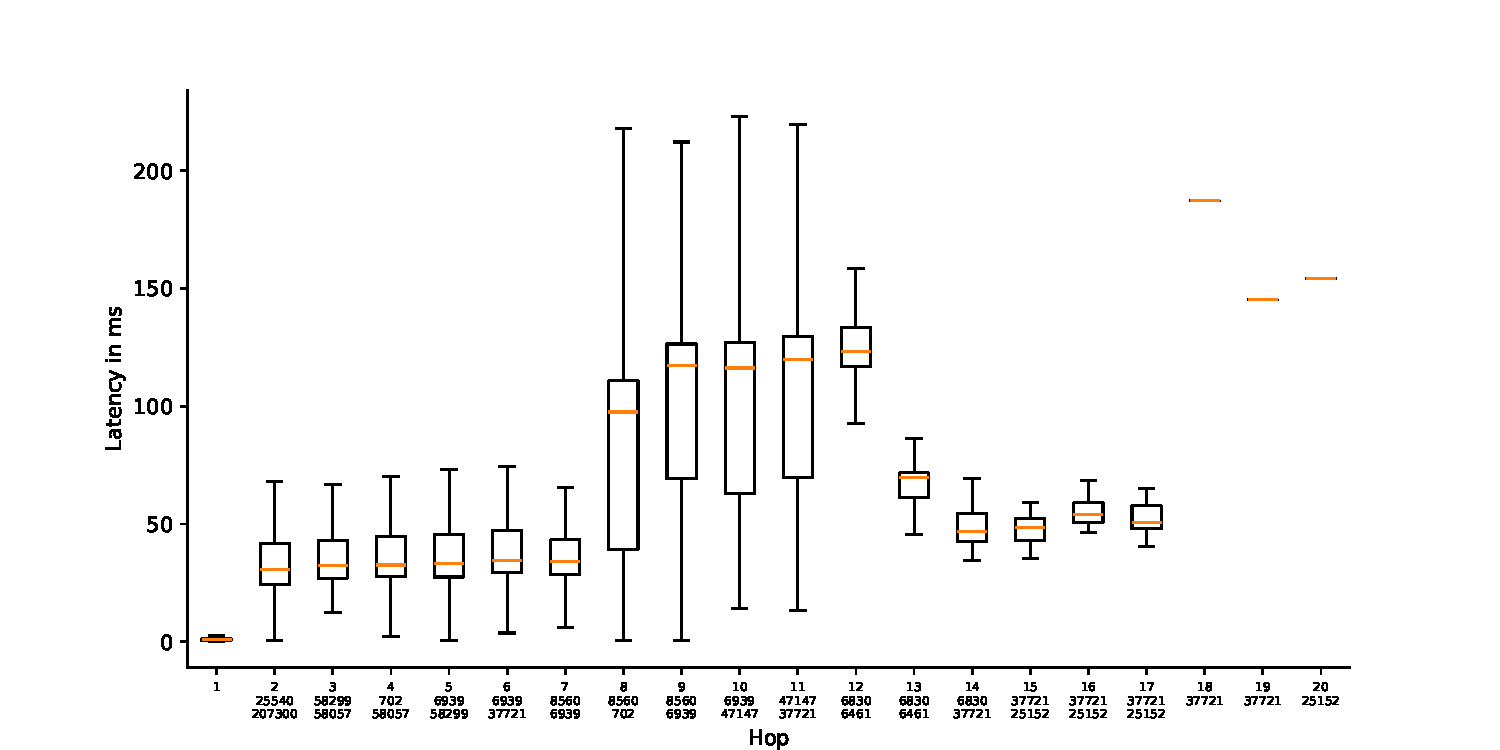
\includegraphics[width=\linewidth]{chapters/4-results/traceroute/img/latency-per-hop-FR-5001.pdf}
		\caption{France}
	\end{subfigure}
	\begin{subfigure}[b]{\linewidth}
		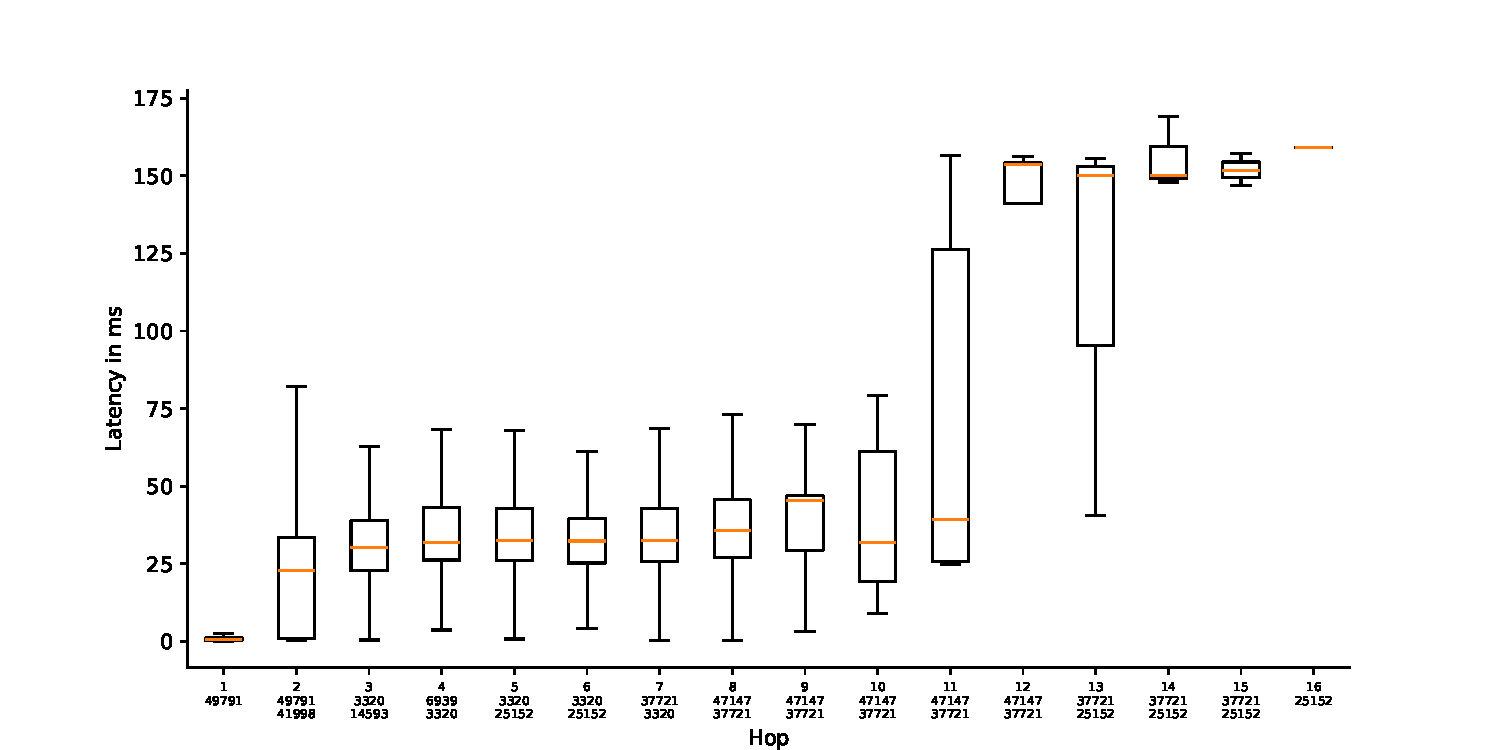
\includegraphics[width=\linewidth]{chapters/4-results/traceroute/img/latency-per-hop-DE-5001.pdf}
		\caption{Germany}
	\end{subfigure}
	\caption{Average Latency per Hop in France and Germany}
	\label{fig:latency-change-per-hop-2}
\end{figure}

One can see that overall each hop increases the RTT slightly, but in most cases
there is a hop that strongly increases the RTT. We assume that this usually is
the hop from the entry into the satellite constellation toward the \ac{GS}. We
also observe that the strong increase sometimes appears in a later hop (e.g.,
in Figure~\ref{fig:latency-change-per-hop-1-ca}). Therefore, we looked at the
\ac{ASN} for each of the hops. We list the most frequent and, if it exists,
also the second most frequent \ac{ASN} under the hop. The \ac{ASN} is acquired
by using \href{https://ipinfo.io/}{IPinfo} data for IPs given by each hop. The
\ac{ASN} allows determining, which autonomous system manages most of the
traffic. Therefore, we can determine whether Starlink is part of the traffic,
which does not seem to be the case for most plots. Usually, Starlink
(\ac{ASN}14593) is not part of the trace after the fifth hop at latest.
Therefore, we assume other factors are responsible for the strong increase at
later hops, i.e., they are not caused by Starlink.

\begin{takeaway}{Starlink Routing Influence on Latency}
	Starlink causes a spike in latency in the first hop(s), because it
	routes through their satellite constellation. There are also later
	spikes in latency, but we do not assume Starlink being responsible for
	that.
\end{takeaway}
